\documentclass[a4paper,twoside]{article}
\usepackage[T1]{fontenc}
\usepackage[bahasa]{babel}
\usepackage{graphicx}
\usepackage{graphics}
\usepackage{float}
\usepackage[cm]{fullpage}
\pagestyle{myheadings}
\usepackage{etoolbox}
\usepackage{setspace} 
\usepackage{lipsum} 
\setlength{\headsep}{30pt}
\usepackage[inner=2cm,outer=2.5cm,top=2.5cm,bottom=2cm]{geometry} %margin
% \pagestyle{empty}

\makeatletter
\renewcommand{\@maketitle} {\begin{center} {\LARGE \textbf{ \textsc{\@title}} \par} \bigskip {\large \textbf{\textsc{\@author}} }\end{center} }
\renewcommand{\thispagestyle}[1]{}
\markright{\textbf{\textsc{AIF184001 \textemdash Rencana Kerja Skripsi \textemdash Sem. Genap 2022/2023}}}

\newcommand{\HRule}{\rule{\linewidth}{0.4mm}}
\renewcommand{\baselinestretch}{1}
\setlength{\parindent}{0 pt}
\setlength{\parskip}{6 pt}

\onehalfspacing
 
\begin{document}

\title{\@judultopik}
\author{\nama \textendash \@npm} 

%tulis nama dan NPM anda di sini:
\newcommand{\nama}{Bosnich Timothy Bonsaleng}
\newcommand{\@npm}{2017730086}
\newcommand{\@judultopik}{Pemvisualisasi Hasil Penelitian Area Hijau Kelurahan} % Judul/topik anda
\newcommand{\jumpemb}{1} % Jumlah pembimbing, 1 atau 2
\newcommand{\tanggal}{06/03/2023}

% Dokumen hasil template ini harus dicetak bolak-balik !!!!

\maketitle

\pagenumbering{arabic}

\section{Deskripsi}
Penelitian yang telah dilakukan oleh Dr.Veronica S.Moertini, Fritz H. Hutapea SKom, dan Juan A. Kusjadi menghasilkan data area hijau dari citra satelit pada Kota Bandung yang dibagi menjadi beberapa kelurahan atau kecamatan Kota Bandung. Citra satelit sendiri merupakan gambar dari bumi yang didapatkan satelit. Hasil dari penelitian terdiri dari area hijau untuk 149 kelurahan di 30 kecamatan kota Bandung dan telah selesai dilakukan perhitungan.\\

\begin{figure}[h]
	\centering
	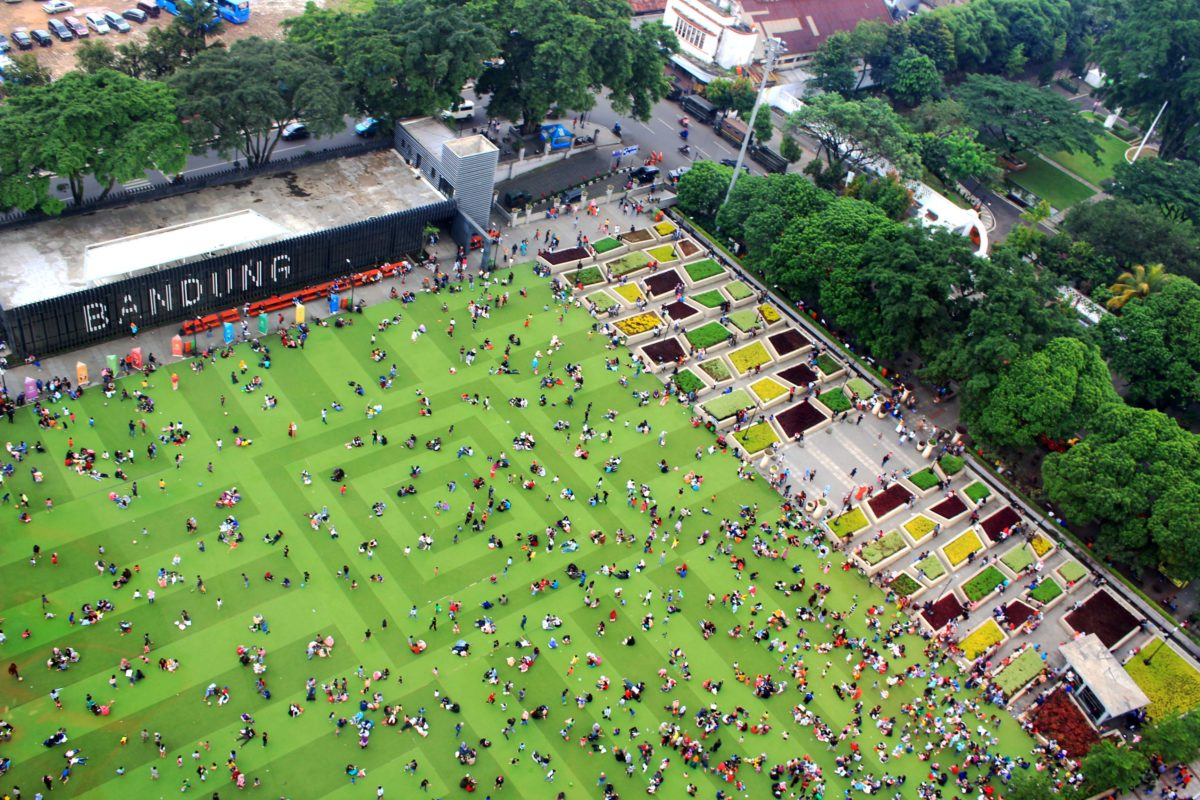
\includegraphics[width=0.5\textwidth]{ruang terbuka hijau.jpg}
	\caption{Contoh Ruang Terbuka Hijau}
\end{figure}
 
Pada Skripsi ini, akan dibangun sebuah laman web yang bertujuan untuk pemvisualisasian dari hasil penelitian area hijau Kota Bandung. Laman web yang akan dibangun harusnya dapat diakses melalui komputer atau laptop,handphone bersistem android ataupun iOS. Dan akan dibantu dengan menggunakan \emph{Framework} Laravel, sehingga memudahkan pengembang untuk membangun perangkat lunak. Dengan adanya laman web pemvisualisasian ini memudahkan pengguna untuk mengetahui area-area hijau yang ada pada Kota Bandung.

\section{Rumusan Masalah}
Rumusan masalah yang muncul berdasarkan deskripsi yang sudah dibahas
adalah sebagai berikut:
\begin{itemize}
	\item Bagaimana membuat sebuah laman web interaktif yang dapat membandingkan dua buah kelurahan atau kecamatan Kota Bandung?
	\item Bagaimana cara pengguna untuk membandingkan atribut-atribut dari kelurahan atau kecamatan Kota Bandung?
	\item Bagaimana cara mengekstraksi data citra satelit pada HDFS?
\end{itemize}

\section{Tujuan}
Tujuan dari skripsi ini adalah sebagai berikut :
\begin{itemize}
	\item Membuat sebuah laman web interaktif yang dapat membandingkan dua buah kelurahan.
	\item Pengguna dapat memilih kecamatan / kelurahan untuk sisi kiri dan kanan, untuk membandingkan atributnya.
	\item Data citra satelit yang didapatkan digunakan untuk memenuhi kebutuhan pada laman web yang dibangun.
\end{itemize}

\section{Deskripsi Perangkat Lunak}
Laman web akan memvisualisasikan hasil dari area hijau Kota Bandung. Fitur-fitur dari laman web akan memudahkan pengguna untuk melihat area hijau dari Kota Bandung berdasarkan kelurahan atau kecamatan. Setiap kelurahan atau kecamatan akan memiliki atribut-atribut sendiri.

Laman Web akhir yang akan dibuat memiliki fitur minimal sebagai berikut:
\begin{itemize}
	\item Pengguna dapat memilih kecamatan atau kelurahan yang ingin dilihat.
	\item Pengguna dapat melihat Luas Wilayah dari kecamatan atau kelurahan yang dipilih.
	\item Pengguna dapat melihat Luas Area Hijau dari kecamatan atau kelurahan yang dipilih.
	\item Pengguna dapat melihat kebutuhan area hijau dari kecamatan atau kelurahan yang dipilih.
	\item Pengguna dapat melihat gambaran citra satelit dari kecamatan atau kelurahan yang dipilih.
	\item Pengguna dapat mengakses ke laman \emph{Google Maps} untuk kecamatan atau kelurahan yang dipilih.
	\item Pengguna dapat gambar luas area hijau dari kecamatan atau kelurahan yang dipilih.
		
\end{itemize}

\section{Detail Pengerjaan Skripsi}
Bagian-bagian pekerjaan skripsi ini adalah sebagai berikut :
	\begin{enumerate}
		\item Melakukan survei kepada Fritz H. Hutapea SKom dan Juan A. Kusjadi terkait penenilitiannya
		\item Melakukan pengumpulan data hasil penelitian
		\item Melakukan studi literatur dan studi eksplorasi mengenai framework Apache Hadoop
		\item Mempelajari ekstraksi data citra satelit yang disimpan pada HDFS
		\item Mempelajari bahasa pemrograman php, html, css dan cara menggunakan \emph{framework} laravel.
		\item Mempelajari kebutuhan laman web.
		\item Melakukan analisis kebutuhan laman web.
		\item Melakukan perancangan antar muka laman web.
		\item Membangun laman web bedasarkan \emph{framework} Laravel.
		\item Melakukan pengujian pada laman web.
		\item Menulis dokumen skripsi.
	\end{enumerate}

\section{Rencana Kerja}
Rincian capaian yang direncanakan di Skripsi 1 adalah sebagai berikut:
\begin{enumerate}
\item Melakukan survei kepada Fritz H. Hutapea SKom dan Juan A. Kusjadi terkait penenilitiannya
\item Melakukan pengumpulan data hasil penelitian
\item Melakukan studi literatur dan studi eksplorasi mengenai framework Apache Hadoop
\item Mempelajari ekstraksi data citra satelit yang disimpan pada HDFS
\item Mempelajari bahasa pemrograman php, html, css dan cara menggunakan \emph{framework} laravel.
\item Mempelajari kebutuhan laman web.
\item Melakukan analisis kebutuhan laman web.
\item Melakukan perancangan antar muka laman web.
\end{enumerate}

Sedangkan yang akan diselesaikan di Skripsi 2 adalah sebagai berikut:
\begin{enumerate}
\item Membangun laman web bedasarkan \emph{framework} Laravel.
\item Melakukan pengujian pada laman web.
\item Menulis dokumen skripsi.
\end{enumerate}

\vspace{1cm}
\centering Bandung, \tanggal\\
\begin{figure}[h]
	\centering
	
\includegraphics[width=0.3\textwidth]{tandatangan.jpg}
\end{figure}
\nama \\ 
\vspace{1cm}

Menyetujui, \\
\ifdefstring{\jumpemb}{2}{
\vspace{1.5cm}
\begin{centering} Menyetujui,\\ \end{centering} \vspace{0.75cm}
\begin{minipage}[b]{0.45\linewidth}
% \centering Bandung, \makebox[0.5cm]{\hrulefill}/\makebox[0.5cm]{\hrulefill}/2013 \\
\vspace{2cm} Nama: \makebox[3cm]{\hrulefill}\\ Pembimbing Utama
\end{minipage} \hspace{0.5cm}
\begin{minipage}[b]{0.45\linewidth}
% \centering Bandung, \makebox[0.5cm]{\hrulefill}/\makebox[0.5cm]{\hrulefill}/2013\\
\vspace{2cm} Nama: \makebox[3cm]{\hrulefill}\\ Pembimbing Pendamping
\end{minipage}
\vspace{0.5cm}
}{
% \centering Bandung, \makebox[0.5cm]{\hrulefill}/\makebox[0.5cm]{\hrulefill}/2013\\
\vspace{2cm} Nama: \makebox[3cm]{\hrulefill}\\ Pembimbing Tunggal
}
\end{document}
